\documentclass[a4paper]{article}
\usepackage[slovene]{babel}
\usepackage[utf8]{inputenc}
\usepackage[T1]{fontenc}
\usepackage{graphicx}
\usepackage{marvosym}
\usepackage{amssymb,amsmath}
\title{Upravljanje maloprodajnega prostora}
\author{Leon Horvat, Jernej Banevec \\ Finančni praktikum \\ Finančna matematika, Fakulteta za matematiko in fiziko}
\date{2017}


\begin{document}
\title{%
  Upravljanje omejenega maloprodajnega prostora za osnovne izdelke \\
  \large Kratko poročilo \\}

\author{Jernej Banevec, Leon Horvat}

\maketitle

\pagebreak

\section{Uvod}


Maloprodajne trgovine imajo veliko izbiro izdelkov, ki jih lahko vključijo v svojo ponudbo, hkrati pa so omejeni s prostorom v posamezni trgovini. Lahko se odločijo, da bodo imeli več različnih produktov z manjšimi zalogami na policah in posledično pogostejšim polnjenjem polic ali pa manj produktov z večjimi zalogami. Nepravilna izbira lahko vodi v nižji dobiček. Trgovci se morajo pri upravljanju maloprodajnega prostora odločiti, katere izdelke vključiti v svojo ponudbo ter optimizirati velikost zalog na policah in urnik njihovega polnjenja. Ti dve odločitvi sta tesno povezani, zato jih moramo obravnavati sočasno. 


Pri analizi problema se bova osredotočila na trgovine, ki imajo v svojo ponudbo vključene izdelke z dolgo življenjsko dobo in stabilnim povpraševanjem. 


\vspace{4 mm}

\begin{figure}[h]
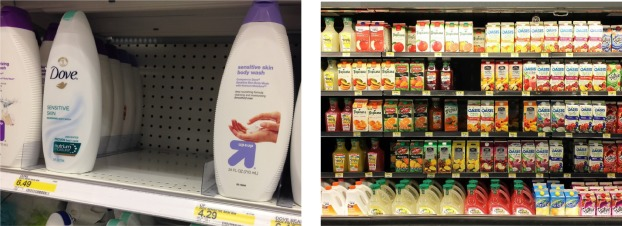
\includegraphics [scale = 0.8]{zgled-strategij}
\caption{Primer strategije dodeljenega prostora in strategije skupnega prostora}
\centering
\end{figure}

Za zgled vzemimo 2 izdelka X in Y, ki imata oba enako velikost 1. Namenimo jima 10 enot prostora. Zalogi obeh se obnavljata na 6 dni. Če obnovimo obe zalogi hkrati, torej prvi dan, prostora na polici ni dovolj glede na povpraševanje izdelka. Če pa zalogo drugega obnovimo prvi dan, prvega pa četrti dan, potrebujemo manj prostora in 10 enot zadostuje povpraševanju obeh izdelkov. Opazimo, da pri uporabi strategije skupnega prostora porabimo manj prostora, vendar je potrebna koordinacija polnjenja zalog izdelkov, ki si delijo prostor.

\begin{figure}[ht]
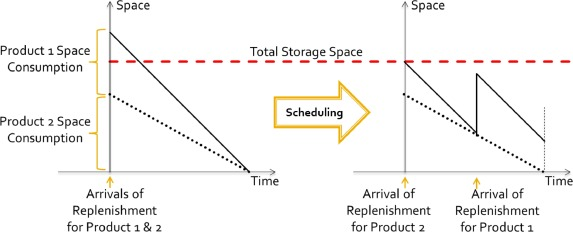
\includegraphics [scale = 0.8]{primerjava-strategij}
\caption{Poraba prostora strategij}
\end{figure}


\section{Modeliranje problema}



Definirajmo:
\begin{itemize}
\item parametre:
\begin{itemize}
\item $ d_i $: prvotna stopnja povpraševanja po izdelku $i$,
\item $ w_{ij}$: delež povpraševanja izdelka $j$ prenesenega na izdelek $i$, če $j$-tega izdelka ni v ponudbi; $w_{ii} = 1$,
\item $ v_i $: dobiček pri $i$-tem izdelku,
\item $ h_i $: strošek hranjenja izdelka na polici,
\item $ k_i $: cena polnjenja izdelka $i$, 
\item $ \theta_i $: koeficient količine varnostne zaloge izdelka $i$.
\end{itemize}

\item odločitvene spremenljivke:
\begin{itemize}
\item $ y_i $: indikator, ki nam pove, ali je izdelek $i$ vključen v ponudbo,
\item $ Q_i $: število naročenih izdelkov $i$.
\end{itemize}

\item pomožne spremenljivke:
\begin{itemize}
\item $ x_{ij} $: indikator substitucije iz izdelka $j$ na izdelek $i$; $x_{ij} = y_i (1-y_j)$, če $j \ne i$ in $x_{ij} = y_i$, če  $j = i$,
\item $ s_i $: končna efektivna stopnja povpraševanja po $i$-tem izdelku; $s_i = y_i (d_i + \sum_{j \ne i} w_{ij} d_j (1-y_j)) = \sum_j  w_{ij} d_j x_{ij}.$
\end{itemize} 
\end{itemize}
\end{document}